\documentclass[11pt,oneside,a4paper]{article}
\usepackage{color}
\usepackage{setspace}
\usepackage{graphicx}
\usepackage{geometry}
\usepackage{amsmath}
\usepackage{bm}
%\renewcommand{\thesection}{\Roman{section}}
%\renewcommand{\thesubsection}{\arabic{subsection}} 
\usepackage{enumitem}
\geometry{
 a4paper,
 total={210mm,297mm},
 left=30mm,
 right=30mm,
 top=25mm,
 bottom=25mm,
 }
\usepackage{hyperref}
\hypersetup{
    colorlinks=true, %set true if you want colored links
    %linktoc=all,     %set to all if you want both sections and subsections linked
    linkcolor=black,  %choose some color if you want links to stand out
}

\begin{document}
\title{\vspace{+2.0cm}  LEVEL-2 PIPELINE SOFTWARE FOR ASTROSAT CADMIUM ZINC TELLURIDE IMAGER (CZTI)\\ USER GUIDE}
\author{Dipankar Bhattacharya (IUCAA, Pune), Mithun N P S (PRL, Ahmedabad),\\ 
Ajay Vibhute (IUCAA, Pune), Mayuri Shinde (IUCAA, Pune), Rakesh Khanna A(TIFR, Mumbai),\\
Tanul Gupta (SAC, Ahmedabad), Preeti Tahliani (SAC, Ahmedabad), \\
Arvind K Singh (SAC, Ahmedabad)}
\date{08 March 2018}
\maketitle

\newpage
\section*{Revision History}
Release 1.0  03 June 2016   initial release  DB \\
Release 1.1 05 October 2016 DB/Mithun \\
Release 2.0 06 October 2017 DB/Ajay
\begin{itemize}
	\item cztimage: Applied corrections for the detector and mask misalignment
	\item cztbindata: Added functionality to compute livetime for fractional binsize
	\item cztpha2energy: Added functionality to process events in chunk
	\item cztdatasel: Minor changes to header keywords
	\item other: Minor bug fixes
\end{itemize}
Release 2.1 08 March 2018 DB/Ajay/Mayuri
\begin{itemize}
	\item cztbindata: Bug fixes in fractional livetime correction
	\item cztdatasel: Fixed a bug in calculation of exposure time
	\item cztpipeline: Added functionality to run pipeline in stages
	\item other: Added a version number to the header of the output file.
\end{itemize}
\newpage

\tableofcontents

\newpage

\section{Introduction}

%\textcolor{red}{Introduction may be rewritten in the context of the scope of this document}


The Cadmium  Zinc Telluride Imager  (CZTI)  on-board  ASTROSAT  is a Coded Mask Imaging 
camera working in the energy range 15 to 150 keV.  The detector is an array of a pixellated CZT  
detectors, and the Coded Mask is composed of a collection of pseudo noise Hadamard coded 
Uniformly Redundant Array (URA) patterns.   The instrument  is  configured  as   four   independent 
quadrants,  each  with 16  detector modules.   Each detector module has 256 pixels. There  are 
collimator  slats   surrounding  every  detector  module  and   the   Coded   Aperture  Mask  is  placed  
above   the   collimator.  The instrument operates in event mode, wherein the time, energy and
pixel coordinates of each photon event is recorded in the data.  There is a CsI Veto detector under 
the CZT modules.  If an event recorded in the Veto occurs within a certain small time window of 
any CZT event, then the latter is tagged with a Veto flag.  The instrument also contains Alpha-tagged 
calibration sources, which generate 60 keV photons simultaneously with an Alpha particle.  CZT 
events that fall within a defined time window of any alpha detection are marked with an Alpha tag
in the recorded data.

Although the CZTI could be configured to work in a variety of modes, in normal course of operation
data are acquired in only three of them.  Mode M0 (Normal Mode) would contain the regular event 
mode data. Mode SS (Secondary Spectral Mode) operates in parallel with all other modes, and 
records, once every 100 seconds, accumulated spectral and housekeeping information.  When the
spacecraft passes through the South Atlantic Anomaly, High Voltage in the CZT and Veto detectors
are switched off, and data collected in Mode M9 (SAA mode) wherein no events, but only housekeeping information is recorded once every second.  Data telemetered to ground are accumulated into separate
files for these different modes before delivery.

%\includegraphics{czti}
\section{Overview of CZTI Data and Pipeline}

The  data    received    from    the     CZTI    payload   passes   through     a   series  of  steps   in  a 
processing   pipeline.   Three   major   data    levels  have    been    designated  for     long-term 
storage. These   are:

\subsection*{Level 0}

This     is  the     raw     data    received    from    satellite   telemetry,  which   is  segregated  by 
instrument, along   with    auxiliary   data.   This    data   is  archived    internally  and not 
distributed   for public  use.

\subsection*{Level 1}

This   is  reorganized raw data,   written in  FITS    format  for Astronomical    use.    All auxiliary   
information necessary   for further processing  of  this    data   are  collated    at  this    level   and 
packed  along   with    the respective  science data.   This    data    is  released  via  Astrosat data
archive,   at  first   to  the     Principal   Investigator    (PI)    of  the     corresponding   observing  
proposal    and,    after   a   specified   initial lock    in  period, to  anyone  interested  in  the data.   

\subsection*{Level 2}

This     data    contains    standard    science     products    derived    from    Level   1   data.   Level   2  
data   is   also   in  FITS  format and is   available    for    science use,    with     the    same    
lock-in criteria    and release mechanism   as  the Level   1   data.\\


The  software    to  process     data    from    Level   1   to  Level   2  contains    user    configurable   
elements.        While   a   default     configuration   is  run   at  the     Payload     Operation   Centre 
(POC)   to  create  the automated   Level   2   standard data    products,   the user has   the option  to  
generate     more    customized  products    by  using   the     same    software    with    other  
configuration    settings.       The     Level   2   pipeline    software  is released publicly   for   general
use.      For Input/Output,   the implementation  of  the pipeline    software    makes   use of  
the  CFITSIO     and     the     Parameter   Interface   Library     developed   and     distributed     by  NASA   
High    Energy  Astrophysics  Science Archive Research    Centre  (heasarc.nasa.gov).\\ \\

\noindent The functionality  and usage of  different components of the CZTI    Level   2   pipeline    
software  are  described   in  this    document.


\section{Level-1 Data Content}

The  input to  CZTI level-2 data reduction pipeline is  the  data set  produced   at   Level   1.     The
original data  is received by telemetry at the Indian Space Science Data Centre (ISSDC), during each 
visible pass over Bengaluru, India.  This data is then packaged every download orbit and sent to the 
Payload Operations Centre (POC) for further processing.    At the POC, all the data belonging to an 
Observation ID (ObsID) are then collected together from various orbit-wise packages and a merged
Level 1 product is created for distribution and further analysis.  The Level 2 pipeline analysis procedure 
described below starts from merged Level 1 package, which contains the following files:

\begin{enumerate}

\item {{\bf Science     Data    File}:   a   FITS    file    containing  sequentially    stacked     2048-byte   data   
frames  generated   by  the CZTI    payload.        This    data    is  mode    segregated, i.e.    a   different   
FITS    file    is  generated   for each    distinct    data    mode.}

\item{{\bf Time    Calibration     Table}(.tct):    This     file   contains    a   list    of   time    tags   expressed   in  
CZTI     internal    clock,  Satellite   On  Board   reference   Time    (OBT)   and     Universal   Time  
(UT)    derived from    the SPS units   on  ASTROSAT.       As  all the CZTI    science data    is  tagged  
with    its internal    clock,  the TCT file    is  required    to  correlate   them    with    other   on-board    
events, as  well   as  to  obtain  absolute    timing.}

\item{{\bf Orbit   File}(.orb):   Gives   time-tagged     orbital     position    of  the     satellite   in  terms   of 
geocentric  x,  y,  z   as  a  function  of  time, as well as the corresponding velocity components.}

\item{{\bf Attitude    File}(.att):   Gives   time-tagged     satellite   attitude    information,    in  terms   of 
quaternions  as  well    as  the     RA,     Dec     values  of  the     pointing    directions  of  the     three  
reference   axes    of  the satellite.}

\item{{\bf LBT     Housekeeping    file}(.lbt):   This    gives   a   time-tagged     recording   of  65  different
health parameters   monitored   by  different   sensors on  the CZTI.}

\item{{\bf MCAP file}(.mcap.xml): This xml file has information like source observed, start and end time of observation etc.}

\item{ {\bf Make  Filter  file}(.mkf):  This    file    collects    together    the time    series  of  a   number  of  
selected     parameters,     including   health  parameters,     Sun     angle,  Earth   angle,  charged    
particle    count   etc,    based   on  which   the quality of  data    obtained    can be  assessed.}

%\item{\textcolor{red}   {Good    Time    Interval    (GTI)   file:   A   list    of  time    intervals   during  which   the     data   
%acquired    may be  considered  good     for    scientific  purposes,   arrived at  on   the    basis   of  
%MKF file    parameters  and pre-set thresholds.}}

%\item{\textcolor{red}    {Bad Time     Interval    (BTI)   file:  A   complement  of  the GTI file,   this    file    records the 
%reason   for    data    acquired    in  any  time   interval    being   considered  not  fit     for    scientific  
%use.}}

\end{enumerate}

\section{Level-2 Pipeline Work flow}

\begin{figure}[]
    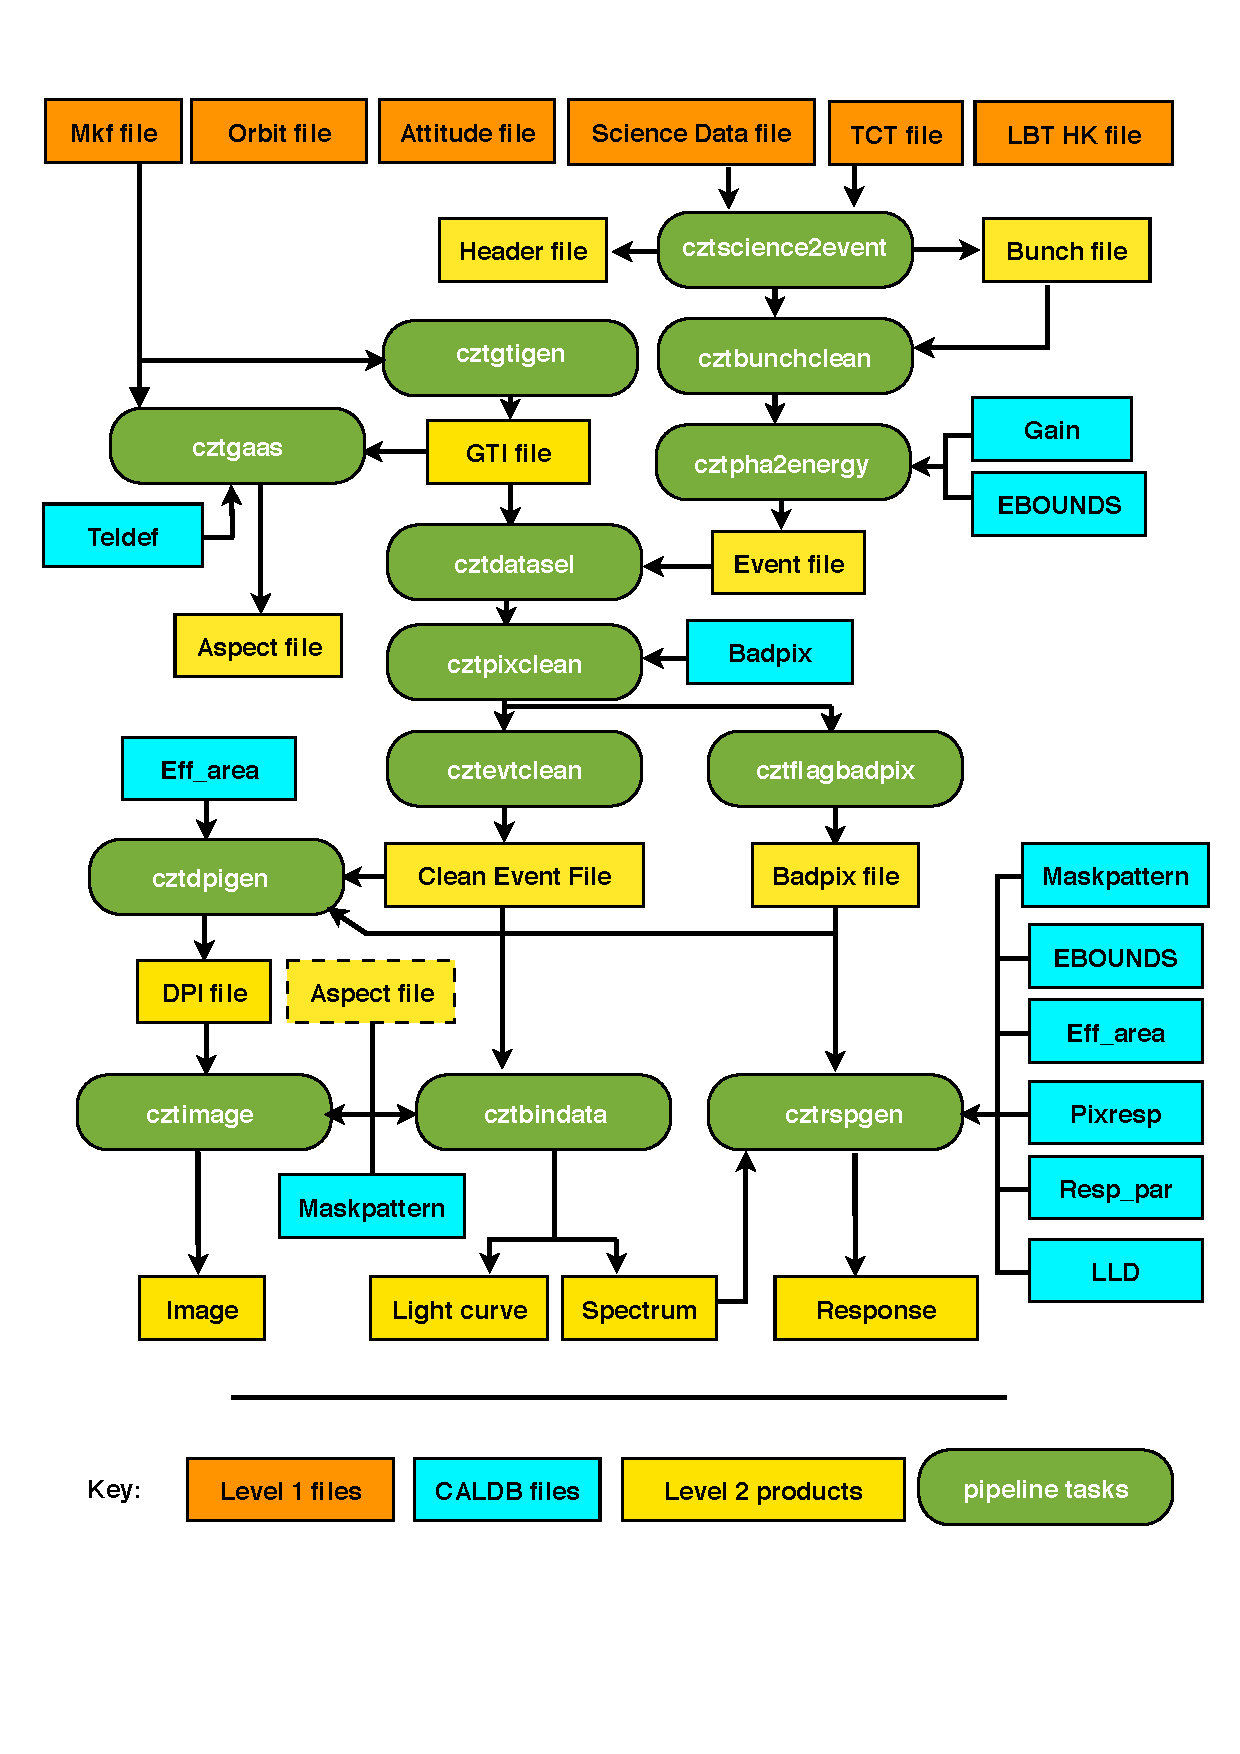
\includegraphics[width=\textwidth]{flowchart_userguide}
    \caption{Level-2 pipeline work flow.}
    \label{flowchart}
\end{figure}

CZTI level-2 data reduction pipeline is organized into different modules for each specific 
task. In figure~\ref{flowchart}, work flow of the pipeline is shown. Table~\ref{task_table} 
summarizes the tasks performed by various software modules.  

Data reduction for CZTI is performed in three stages. Each of these stages involves 
execution of several tasks of the pipeline. 

\begin{itemize}

    \item{{\bf Stage 1}: Generation of event file and calibration. In this stage event file is generated
from level 1 data, gain offset corrections are applied and multi hit events are removed.}

\item{{\bf Stage 2}: Selection of data and cleaning. In this stage events are selected based on Good
Time Interval and noisy pixel events are removed from the data.
}

\item{{\bf Stage 3}: Generation of science products. In this last stage,DPI, image, spectrum, light curve and response
        matrix are generated.
}
\end{itemize}

The pipeline tasks can either be executed individually or by using the {\bf cztpipeline} module 
which allows the user to run required stages of the pipeline tasks.

\begin{table}[]
\begin{center}
\begin{tabular}{|l |l| l|}
\hline
Sl No & Module name & Functionality \\ \hline
1 & cztscience2event &  \begin{tabular}{@{}l@{}}
a) Extraction    and     decoding    of  level-1 science data\\    
\hspace{14pt}into    events\\
b) Mapping   of  quadid,    detid  and  pixid  to detx,dety\\
c) Mapping  of  12  bit PHA to  10  bit PHA channels \\
d) Time calibration \\
e) Recording    of  temperature history\\
\end{tabular} \\ \hline
2 & cztbunchclean & Clean the event file by identifying and removing bunches\\ \hline
3 & cztpha2energy & 
Convert PHA value to PI and write to event file \\ \hline
4 & cztgtigen & Generate GTI based on current gti, mkf and user input\\ \hline
5 & cztgaas & Compute time dependent and average aspect of CZTI\\ \hline
6 & cztdatasel & Select events based on gti\\ \hline
7 & cztpixclean & Identify noisy pixels and detectors and remove noisy events\\ \hline
8 & cztflagbadpix & Combine bad pixel list from multiple sources, if required\\ \hline
9 & cztevtclean & Select events based on veto and alpha tags\\ \hline
10 & cztdpigen & Generate Detector Plane Image from clean event file\\ \hline
11 & cztimage & Create image using Fast Fourier Transforms\\ \hline
12 & cztbindata & Generate light curve/spectrum\\ \hline
13 & cztrspgen & Generate response matrix file\\ \hline
\end{tabular}
\end{center}
\caption{Summary of tasks in CZTI level-2 pipeline}
\label{task_table}
\end{table}


\newpage

\section{Download and Installation}

CZTI data reduction pipeline is available in AstroSat Science Support Cell (SSC) website 
in the link given below:\\

\url{http://astrosat-ssc.iucaa.in/uploads/czti/czti_pipeline_20180308_V2.1.tar} \\

\noindent Please follow the instructions below to install the software. 

\subsection*{Pre-Requisites}
    OS: Linux/Unix (CentOS-5.8+, Ubuntu 14.04+, OS X 10.10+, Scientific Linux 6.5+)\\
    Compiler: gcc (GCC) 4.4+, gfortran, Perl 

\subsection*{Installation Instructions}

\noindent 1. Run the command 'bash' to change the shell to bash shell \\ 

\noindent 2. Untar the package.
\begin{verbatim}
    tar -xvf czti_pipeline_20180308_V2.1.tar
\end{verbatim}

    This will create a directory named "czti\_pipeline" \\ 
 
\noindent 3. Set following environment variables in  \textasciitilde/.bashrc file

\begin{verbatim}
    as1czt : Absolute path of czti folder( under "czti_pipeline/czti") 
    PFILES : Absolute path of paramfiles folder 
    PATH   : Absolute path of bin directory where all executables are placed 
    LD_LIBRARY_PATH : Path to shared libraries 
\end{verbatim}

by adding following lines to  \textasciitilde/.bashrc file
\begin{verbatim}

    export as1czt=<path to czti directory>
    export PFILES=$as1czt/paramfiles
    export PATH=$as1czt/bin:$as1czt/scripts:$PATH
    export GLOG_log_dir=$as1czt/log
    export CZTI_templates=$as1czt/templates
    export PERL5LIB="$as1czt/lib/":$PERL5LIB    
    export LD_LIBRARY_PATH=$LD_LIBRARY_PATH:$as1czt/lib
	ulimit -s 65532
\end{verbatim}


OS X users: In addition to above lines, specify DYLD\_LIBRARY\_PATH by adding the following line to \textasciitilde/.bashrc.
\begin{verbatim} 
    export DYLD_LIBRARY_PATH=$DYLD_LIBRARY_PATH:$as1czt/lib
\end{verbatim}

\noindent 4. CALDB installation: 
    Untar  caldb\_goodfiles\_as1\_czti*.tar.gz (available at the ASSC website) in a preferred location or under existing CALDB directory if caldb installation for other missions are present. It should produce directory structure data/as1/czti/, under which there would be caldb.indx file and calibration files.

Export the CALDB path by adding the below line in  \textasciitilde/.bashrc file
\begin{verbatim} 
    export CALDB=<path to CALDB directory>
\end{verbatim}

\noindent 5. Execute the following commands in bash
\begin{verbatim}    
    source ~/.bashrc
    cd $as1czt
    cd ../
    ./InstallLibs
    cd $as1czt
    make
    cd scripts
    chmod +x cztpipeline
\end{verbatim}
The installation procedure is now complete.  
    	

\section{Description of \emph{cztpipeline}}

\emph{cztpipeline} is a perl script which executes the tasks of CZTI data analysis 
pipeline in sequence. The user can decide to run specific stages of data analysis and 
also can configure many of the parameters of individual tasks of the pipeline.

Input parameters of \emph{cztpipeline} are described below. The default value of 
each of the parameters is given in square brackets. Note that many of these parameters 
are hidden and unless the user defines these parameters as input arguments in command 
line, the default values would be used. For further details of the parameters of specific tasks, 
please refer to the subsequent sections describing the software modules. 

%\subsection*{\emph{Common parameters}}

\subsection*{l1dir~[]}
    Path to level 1 data directory. This should point to the top level directory 
of level 1 extracted from the downloaded archive file. Please make sure not to change the 
name of the directory.
\subsection*{l2dir~[]}
    Location of level 2 data directory. \emph{cztpipeline} will create a level 2 
data directory under this location.
\subsection*{entrystage~[1]}
    Entry stage for analysis. As described earlier, the data reduction has 
three distinct stages. This parameter defines the start stage of analysis. 
Minimum acceptable value is one and maximum is three.
\subsection*{exitstage~[3]}
    Exit stage for analysis. Exit stage can be one, two or three, but the value 
should not be less than the entry stage. If user wishes to perform only one stage, 
say stage 3, both entry and exit stages should be set as three. Also note that 
execution of any stage requires products from earlier stages.
By default all three stages of the pipeline would be executed. 
\subsection*{clobber~[yes]}
    Replace existing files. If clobber is set to yes, files existing in the 
location if any would be replaced. By defualt clobber is set to yes. 
\subsection*{history~[yes]}
    Write history to file header. This keyword controls writing of history parameters 
to header of the output FITS files. Users are adviced to keep it at the default.
\subsection*{debug~[no]}
    Run in debug mode. This parameter controls chatter level. If set, the pipeline 
tasks would print debugging information.
\subsection*{eboundsfile~[CALDB]}
    Ebounds file defining nominal energy range of pulse invariant channels. If set 
to CALDB, pipeline will pick the file from caldb distribution.
\subsection*{gainfile~[CALDB]}
    Gain and offset file, which contains temperature dependant gain and offset values 
of detector pixels that are used to convert PHA to PI channels.If set 
to CALDB, pipeline will pick the file from caldb distribution.
\subsection*{effareafile~[CALDB]}
    Effective area file which contains effective area of detector pixels. If set 
to CALDB, pipeline will pick the file from caldb distribution.
\subsection*{lldfile~[CALDB]}
    Lower Level Discriminator channels of pixels, which defines the lowest 
responsive channel of each pixel. If set 
to CALDB, pipeline will pick the file from caldb distribution.
\subsection*{badpixfile~[CALDB]}
    List of bad pixels, which has flags of disabled and spectroscopically bad pixels.
If set 
to CALDB, pipeline will pick the file from caldb distribution. 
\subsection*{maskfile~[CALDB]}
    Coded mask pattern file, which defines the coded aperture mask pattern. If set 
to CALDB, pipeline will pick the file from caldb distribution.
\subsection*{camgeomfile~[CALDB]}
    Camera geometry definition file, which defines the geometry of the instrument 
including the collimators and other structures. If set 
to CALDB, pipeline will pick the file from caldb distribution.
\subsection*{respparfile~[CALDB]}
    Response parameter file having parameters of response model for pixels. This includes 
electron and hole mobility values, resolution etc. If set 
to CALDB, pipeline will pick the file from caldb distribution.
\subsection*{pixrespfile~[CALDB]}
    Pixel wise redistribution matrix file, which stores pre-computed redistribution 
matrices for groups of pixels. If set 
to CALDB, pipeline will pick the file from caldb distribution.
\subsection*{\emph{Inputs of cztscience2event}}
    
\subsection*{sc2evt\_buffersize~[100000]}
    Buffer size for cztscience2event. The task cztscience2event reads 
data packets from level 1 directory and extracts events to output event file. 
This parameter controls the number of packets to be read at a time. User 
can change this parameter depending upon the memory available.
\subsection*{bigendian~[yes]}
    Whether bigendian. 
\subsection*{\emph{Inputs of cztbunchclean}}

\subsection*{bunchdeftime~[30]}
    Bunch definition time. This parameter defines time difference between 
events which should be assigned as same bunch. Refer to section on cztbunchclean 
for more details.
\subsection*{bunch\_length\_thresh~[20]}
    Threshold value for bunch length, which is defined as  the number of events in a bunch. 
This parameter distinguishes short and long bunches.
\subsection*{skipT1~[0]}
    skipT1 parameter for bunchclean, which defines the time range for 
discarding events after every bunch.
\subsection*{skipT2~[0.001]}
    skipT2 parameter for bunchclean, which defines the time range for 
discarding events in the module after short bunches.
\subsection*{skipT3~[0.001]}
    skipT3 parameter for bunchclean, which defines the time range for 
discarding event in the quadrant after long bunches.
\subsection*{livetime\_binsize~[1]}
    Time binsize for livetime calculation. Multi-hits events (bunches) cause reduction in 
livetime. cztbunchclean computes livetime for each quadrant, and this parameter defines 
the size of time bin for which live time would be computed. 
 
%\subsection*{Inputs of cztpha2energy}

\subsection*{\emph{Inputs of cztgtigen}}

\subsection*{mkfthresholdfile~[\$as1czt/paramfiles/mkfThresholds.txt]}
    Threshold file for MKF parameters for GTI selection. This file defines 
thresholds on various parameters in MKF file which would be used for 
generation of Good Time Interval.
\subsection*{usergtifile~[-]}
    Optional user GTI file. User can provide additional GTI file an input 
to select data in desired intervals. This file should be standard GTI FITS 
file with binary extension named GTI with two columns START and STOP defining 
start and stop times of the intervals.

%\subsection*{Inputs of cztgaas}

\subsection*{\emph{Inputs of cztdatasel}}

\subsection*{gtitype~[QUAD]}
    GTI selection type. Valid inputs are `QUAD' and `COMMON'. QUAD type 
generated GTI specific to each quadrant, whereas if COMMON is set, the 
output GTI would be intersection of Good Time intervals of all quadrants. 
In case the user wishes to add data from all four quadrants, `COMMON' GTI 
type is suggested.

\subsection*{\emph{Inputs of cztpixclean}}
    
\subsection*{noisypix\_nsigma~[5]}
    Noisy pixel threshold. This parameter defines the definition of noisy  
pixels. Pixels with counts beyond noisypix\_nsigma standard deviation from 
mean pixel count rate are removed.  
\subsection*{dettbinsize~[1]}
    Detector light curve bin size for pixclean. This defines bin size 
for light curves used for rejection of noisy times of detectors. 
\subsection*{pixtbinsize~[1]}
    Pixel light curve bin size for pixclean. This defines bin size 
for light curves used for rejection of noisy times of pixels.
\subsection*{detcount\_threshold~[35]}
    Detector count threshold. Time bins with detector counts 
beyond this threshold are rejected.
\subsection*{pixcount\_threshold~[2]}
    Pixel count threshold. Time bins with pixel counts 
beyond this threshold are rejected.
\subsection*{writedblevt~[no]}
    Whether write double event file. If this parameter is set to yes, double 
event file with Compton scattered events would be written as additional output.

\subsection*{\emph{Inputs of cztevtclean}}

\subsection*{alphasel~[0]}
    Alpha flag to be selected. If set to zero, cztevtclean rejects events with 
coincident alpha tag. Only alpha tagged events are selected if it is set to one,
which would be useful for calibration only. 
\subsection*{vetosel~[0]}   
    Veto range to be selected. If set to zero, events with coincident events in 
veto detector would be rejected. 
\subsection*{\emph{Inputs of cztdpigen}}

\subsection*{dpi\_badpixthreshold~[0]}
    Threshold of badpixels in DPI generation. Pixels with flag less than or equal to 
this parameter would be used in the generation of Detector Plane Image.
\subsection*{dpi\_timerange~[-]}
    Time range for DPI. Defines the start and end time for generation of 
DPI.
\subsection*{dpi\_energybins~[-]}
    Energy range for DPI. Defines low and high energy limits for events 
to be used in generation of DPI.
\subsection*{\emph{Inputs of cztimage}}
    
\subsection*{image\_inputtype~[DPI]}
    Type of input for cztimage. Defines the type of input to cztimage. 
Vaid options are DPI, DPH, SHADOW.
\subsection*{\emph{Inputs of cztbindata}}

\subsection*{applymaskweight~[yes]}
    Whether to apply maskweights. If set to yes, output spectrum and light curve will 
have mask weighted background subtracted counts. Counts in mask-weighted spectrum are 
"background subtracted counts per unit area of fully illuminated detector plane". If 
this parameter is set to no, spectrum and light curve would contain all events recorded.
 \subsection*{rasrc~[-]}
    Source Right Ascension. Right ascension of source of interest in FOV, given in 
decimal degrees. 
\subsection*{decsrc~[-]}
    Source Declination. Declination of source of interest in FOV, given in 
decimal degrees.
\subsection*{bindata\_badpixthreshold~[0]}
    Badpixel threshold for bindata. Pixels with badpix flag greater than this threshold 
are ignored while generating spectrum and light curve.
\subsection*{bindata\_outputtype~[both]}
    Output type for bindata. Valid options are spec, lc and both.
\subsection*{lc\_timebinsize~[1000.0]}
    Time bin size for light curve in seconds.
\subsection*{lc\_energyrange~[-]}
    Energy range for light curve. Low and high energy limits for events to be used 
for generation of spectrum and light curve.
\subsection*{applyLLD~[yes]}
    Whether to apply LLD cut. If it is set to yes, events below LLD of pixels would be discarded 
while generating outputs.
\subsection*{generate\_eventfile~[yes]}
    Whether generate event file with mask weights. If set to yes, an event file identical to 
input event file with additional columns of mask open fraction and weight would be generated.
\subsection*{bindata\_quadsToProcess~[-]}
    This parameter decides which quadrants to be processed by cztbindata. Note that, in case 
the GTI type of input event file is `QUAD', the spectrum and light curve would be produced for 
each of the quadrants separately and if it is `COMMON' then data from all selcted quadrants will 
be added together.


\section{Description of Software Modules}

%%%%% SCIENCE2EVENT %%%%%%%%%%%%%%%%%%%

\subsection{cztscience2event}

This   module   reads   the   level 1   science   data   file   and   decodes   the   data   packets   into  
events. It  creates  an  event  file  in  FITS  format  with  events  for  each  quadrant  in  different  
extensions. Each event is assigned a calibrated time stamp which is computed using the
time calibration table. Relevant housekeeping information present in headers and detector temperature 
information present in modeSS data are also decoded and written to output files in tabular form.

\subsubsection*{Input}
\renewcommand\labelitemi{{\boldmath$\cdot$}}
\begin{itemize}
\item{Science data file}
\item{Tct file}
\end{itemize}
\subsubsection*{Method}
\begin{itemize}

\item{Read  the  data  packets  from  the  Data Array  column of level 1 science data file into   buffer.}

\item{Decode  each  of  the  2048  byte  data  packet  from  the  buffer  as  per  the  format specified in   
on-board  software document.} 

\item{Read  the  fields  of  the  frame  header.  From  the  values  of  header fields,  get  the  frame  number, 
mode  id,  quad  id,  the  number  of  events  in  the  frame  and  read  the  event  data  accordingly into  an  event  buffer.}

\item{Take  the  time  for  each  event  (fractional  second)  and  the  second  count  value  from  its  frame  
header  and  add  both to  get  the  event  time  in  seconds.  Using  the level 1 TCT  
file,  convert  the  CZTI instrument time  to  UTC  time  using  interpolation.  Record  this  interpolated  time  as  an  
additional  column  in  the  data. }

\item{While decoding the PHA value read only the most significant 10 bits, to get PHA value 
in the range 0-1023.}

\item{Create  the  output  event  file  with  4  extensions  for  four  quadrants  with  extension  names  as  Q0,  
Q1,  Q2 and  Q3}

\item{Create  a  binary  table  in  each  extension  with  columns  time, cztseccnt, cztnticks, pha,  detid,  pixid,
 detx, dety, veto, alpha  and  write  the  decoded events to appropriate extensions.} 

\item{For  each  event  in  4  quadrants,  map  the  quad id, detid  and  pixid  into  (detx,dety)  position 
on each quadrant of CZTI. Write this into corresponding columns of event file.}

\item{Decode Veto spectrum from frame header and write it to Vetospectrum extension of event file.}

\item{Copy all relevant keywords to event file FITS headers.}

\item{Copy the GTI extensions from level 1 science file to the output event file.}

\item{Decode the HK parameters and other information from frame headers and write them to hdr file
as a binary table.}

\item{In case of modeSS frame, decode the spectra and temperature information and write to SSM and TEMP extensions 
of event file and leave the event data extensions empty.}

\end{itemize}
\subsubsection*{Output}
\begin{itemize}
\item{Level 2 event file}
\item{Level 2 header file}
\item{Bunch information file} (see below)
\end{itemize}

%%%%% BUNCHCLEAN %%%%%%%%%%%%%%%%%%%%%%%%

\subsection{cztbunchclean}
Hard X-ray detectors are sensitive to charged particle interactions. Particles 
interacting with the detector lose energy continuously and produce tracks.
Charged particles interacting with the instrument or spacecraft body 
produce secondary particles and X-ray photons, 
which can also deposit energy in the CZTI detectors. 

As CZTI is composed of pixellated detectors, each pixel acts as an independent X-ray detector. 
So one charged particle can produce events in many pixels of CZTI at the same time. We call 
these multi-hit events as `bunches', as they are bunched in time. Such events need to be identified 
and removed from the event file. This module of the level-2 pipeline identifies 
the bunched events and removes them. It also keeps track of the dead time caused by this. 
During the Performance Verification phase, one level of removal of bunched events has been implemented 
in the on-board processing in order to reduce the data volume. Relevant information of 
each bunch of events are encoded along with the other events. 

\subsubsection*{Input}
\renewcommand\labelitemi{{\boldmath$\cdot$}}
\begin{itemize}
\item{Raw event file}
\item{Bunch file}    
\end{itemize}
\subsubsection*{Method}
\begin{itemize}
\item{A bunch is defined as a collection of events occurring within $bunchdeftime ~(30~\mu s)$. Any event
with a difference in time stamp less than or equal to $bunchdeftime$ from its neighbours belongs to the same bunch}
\item{In the current version of on-board software, bunches are identified on-board and only three 
events of a bunch are recorded along with other relevant information of the bunch. Information 
about the bunches are decoded to bunch file produced by cztscience2event}
\item{Each entry in bunch file corresponds 
to one bunch. Read the event file and bunch file to identify the events belonging to the bunch}
\item{Events are assigned flag which denotes how many events are present
in the bunch of the current event. Single events are flagged as one and 
double events are flagged as two}
\item{Remove all events flagged as three or above, only single and double
events are retained. Compute the bunch duration and subtract it from the 
live time for that second, which is initialized to one. Fractional exposure 
of all pixels of the quadrant is also modified.}

\item{There is provision to ignore all events within $skipT1 ~(0 ~s)$ time after the bunch. If it 
is non-zero the events are ignored and live time is modified}

\item{For bunches with events less than or equal to $bunch\_length\_threshold ~(20)$, all events of
the module where the bunch occurred are ignored for $skipT2 ~(0.001~s)$ time after the
end of bunch. If the events in bunch are spread across modules, then the module with the largest number 
of events in the bunch is considered for this. Fractional exposure of the pixels 
of that module and the live time are modified accordingly}

\item{For bunches with events more than $bunch\_length\_threshold ~(20)$, all events
are ignored for  $skipT3 ~(0.001~s)$ time after the end of bunch. Fractional exposure 
of all pixels of the quadrant and the live time are modified accordingly}

\item{Note that all three time parameters are from the end time of the bunch, hence
maximum ignored time is bunch duration plus maximum of the three time parameters.}

\item{Single and double events after this cleaning are written out in the standard
event file format.}

\item{An EXPOSURE extension is added to the output event file where the
fractional exposure of each pixel is stored.}

\item{Live time for each one second interval during the observation is written to 
output live time file}

\end{itemize}
\subsubsection*{Output}
\begin{itemize}
\item{Event file devoid of bunched events}
\item{Live time file}    
\end{itemize}

%%%%%% PHA2ENERGY %%%%%%%%%%%%%%%%%
\subsection{cztpha2energy}
Each  X-ray  photon incident on  the  CZT  
detector produces charge proportional to photon energy, which is measured  as  a  voltage, and  through  the  
Analog to Digital  Converters  it is  recorded  as  a  Pulse Height  Amplitude   (PHA)   channel   value.     
This   software   module   uses   temperature dependent pixel wise calibration  data  
to  estimate  the  nominal  energy  of  the  incident
photon  from  the  recorded  PHA, and  expresses  it  on  a  Pulse Invariant  and  Pixel Invariant  scale,  called  a  PI  channel  value. 

\subsubsection*{Input}
\renewcommand\labelitemi{{\boldmath$\cdot$}}
\begin{itemize}
\item{Event file}
\item{Event file with SS Mode data}
\item{Gain file from caldb}
\item{Ebounds file from caldb}
\end{itemize}
\subsubsection*{Method}
\begin{itemize}

\item{Copy  the  input  event  file  to  output  event  file.}

\item{Query CIF file to get caldb Gain and Ebounds files.}

\item{Add  two  columns,  PI,  and Energy  in  the  output  file.}

\item{Read  the  PHA,  detid  and  pixid  of  each  event.}

\item{Get  the  temperature  of  the  detector  at  event  time  from  the  TEMP  extension 
of SS Mode event file by interpolation. }

\item{Read  Gain  and  offset  at  a  temperature  nearest  to  the  actual  detector
temperature for that event pixel from  the caldb Gain file. }

\item{Compute the energy of event as:
$E = \mbox{\rm gain}*\mbox{\rm PHA} + \mbox{\rm offset}$}


\item{From  Ebounds,  find  to which  PI  bin does the  computed  energy  belong.} 

\item{Write the energy and PI values of the event to respective columns of the 
output file.}

\item{Copy SSM and TEMP extensions from SSM event file to the output modeM0 event file.}

\end{itemize}
\subsubsection*{Output}
\begin{itemize}
\item{Event file with Energy and PI columns added}
\end{itemize}

%%%% GTIGEN %%%%%%%%%%%%%%%%%%%%%%

\subsection{cztgtigen}

During the course of observation, there are time intervals where the data is not 
present due to SAA passage, data transmission loss etc. Also there are intervals 
when the source is occulted by the earth or the angular offset of the source has changed. 
In order to generate science products from such observations, it is important 
to identify such intervals and ignore the data for that duration and to properly 
account for the data gaps.

This task produces GTI file for each quadrant of CZTI based on thresholds on 
various parameters, as well as the GTI present in the event file. It also 
has provision to accept user defined GTIs for specific analysis cases.

\subsubsection*{Input}
\renewcommand\labelitemi{{\boldmath$\cdot$}}
\begin{itemize}
\item{Event file}
\item{MKF file}
\item{MKF threshold file}    
\item{Optional user GTI file}    
\end{itemize}
\subsubsection*{Method}
\begin{itemize}
\item{Read the mkf threshold file which defines the range of various mkf parameters for GTI}
\item{Find time ranges when the all the mkf parameters are within the required ranges to generate GTI 
    based on MKF}    
\item{Read the quadrant wise and common GTIs from the event file}        
\item{Find the intersection of common GTI with the MKF GTI and any other GTI provided by user}
\item{Similarly find the intersection of each quadrant GTI with MKF and user provided GTIs}
\item{Write the output GTIs as different extensions of GTI file}
\end{itemize}
\subsubsection*{Output}
\begin{itemize}
    \item{GTI file}
\end{itemize}

%%%% GAAS%%%%%%%%

\subsection{cztgaas}

In  order  to  find  the  position  and  orientation  of  the  CZTI  field  of  view  
one  needs  to  utilize  the  satellite  aspect  information and  account  for  the alignment  of  
the  CZTI  payload with  respect  to  the  satellite reference  axes which is recorded in the 
telescope definition file. This module computes the time dependent pointing direction of CZTI axes 
as well as the average value.

\subsubsection*{Input}
\renewcommand\labelitemi{{\boldmath$\cdot$}}
\begin{itemize}
\item{Event file}
\item{MKF file}
\item{Teldef file from caldb}
\item{GTI file}
\end{itemize}
\subsubsection*{Method}
\begin{itemize}
\item{Read  the  CZTI  alignment  matrix  elements  from  teldef  file. The  matrix  elements  define  the  
transformation  of  a  vector  (DETX,  DETY,  DETZ)  defined  in  detector  coordinates  to  satellite  
body  coordinates  (SATX,  SATY,  SATZ) }

\item{From  the  MKF  file,  for  every  recorded  sample,  
read  (RA,  Dec)  values  of  the  Yaw,  Roll, Pitch  axes.  
From  these,  derive  their  Direction  Cosines  in  the  Inertial  Coordinate  System.}

\item{Construct  
a  transformation  matrix  from  satellite  body  coordinates  to  the  Inertial  Coordinate  
System (ICS) using the above direction cosines}  

\item{CZTI z-axis is defined by vector [zDET]=(0,  0,  1) and x-axis  by [xDET]=(1,  0,  0)
in czti detector coordinate system.  Find  the  components of these two unit 
vectors in  the  ICS for every sample in the mkf file and record them along with the time stamp in   the   output   CZTI   aspect   array   file.
}

\item{Read the quadrant wise extensions of the GTI file}

\item{Average  the  components  individually  over  the  duration  of  good time intervals, and construct
vectors out of these average components and normalise to obtain  averaged unit vectors $N$ and $T$ respectively.}


\item{Find  the  average  pointing  direction  of  the  CZTI from:
$${\rm DEC} =  \mbox{\rm asin}(N_z); \; {\rm RA}  =  \mbox{\rm atan2}(N_y,N_x) \; \mbox{\rm mod} \;  360 \; \mbox{\rm deg} $$
and the  average  TWIST  angle from:
$${\rm TWIST}=\mbox{\rm atan2}[{T_y  \cos({\rm RA})-T_x  \sin({\rm RA})},{T_z  \cos({\rm DEC})–\sin({\rm DEC})(T_x  \cos({\rm RA})+T_y \sin({\rm RA}))}]$$
}

\item{Record  the  normalized  vectors,  
RA,  DEC  and  TWIST  values  in  the  FITS  header  of  the  Aspect file}

\end{itemize}
\subsubsection*{Output}
\begin{itemize}
    \item{Aspect file}
\end{itemize}

%%%%%%% DATASEL %%%%%%%%%%%%%%%%%

\subsection{cztdatasel}
This pipeline module filters the events in the input event file based 
on GTI file. As each quadrant has an independent GTI, it is possible to 
filter each quadrant data by the respective GTI or filter all quadrants 
with the common GTI. User input GTITYPE which has two possible values 
quad or common, determines this.

\subsubsection*{Input}
\renewcommand\labelitemi{{\boldmath$\cdot$}}
\begin{itemize}
\item{Event file}
\item{GTI file}
\end{itemize}
\subsubsection*{Method}
\begin{itemize}
    \item{If the user defined GTI type is QUAD, read the quadrant wise GTI extensions of the GTI file. Else 
        if the GTI type is COMMON, read the common GTI extension of GTI file}
    \item{Select the events with time stamps which are within the good time intervals}
    \item{Write the selected events to the output event file}
    \item{If gtitype is quad, copy the four quadrant GTIs to the output event file, else copy 
        common GTI to the output file}    
\end{itemize}
\subsubsection*{Output}
\begin{itemize}
    \item{GTI filtered event file}
\end{itemize}

%%%%%%%%% PIXCLEAN %%%%%%%%%%%%%%%%%

\subsection{cztpixclean}
CZTI is composed of 64 detectors each having 256 pixels. Some of these pixels can be 
noisy during the observations. In some cases, a few pixels are consistently noisy for 
substantial duration of the observation, and the events from these pixels need 
to be filtered out. Certain pixels and detectors are noisy for short durations and 
these pixels/detectors need to be ignored for those durations. This pipeline module 
filters the event file for noisy pixels/detectors.

\subsubsection*{Input}
\renewcommand\labelitemi{{\boldmath$\cdot$}}
\begin{itemize}
\item{Event file}
\item{Livetime file from bunchclean}
\item{Badpix file from caldb}
\end{itemize}
\subsubsection*{Method}
\begin{itemize}
\item{Detector Plane Histogram is generated and noisy pixels are identified
by iterative $nsigma~(5)$ clipping. The disabled pixel list from caldb is also
taken into account.}
\item{All events from already designated noisy and dead pixels are ignored.}
\item{Generate detector light curve with bin size $det\_tbinsize~(1~s)$. Ignore events from a
module for a given time bin if counts in that bin is greater than $det\_count\_threshold~(25)$}
\item{Generate pixel light curve with bin size $pix\_tbinsize~(1~s)$. Ignore events from a
pixel for a given time bin if counts in that bin is greater than $pix\_count\_threshold~(2)$}
\item{Fractional exposure time of pixels and live time are modified accordingly.}
\item{Single events and double events are written out in standard event file format
separately. Modified pixel wise fractional exposures are written to the EXPOSURE extension
of both the event files.}
\item{Badpixel file with the dead and noisy pixels flagged is created.}
\item{Modified live time values are written in the output file}
\end{itemize}
\subsubsection*{Output}
\begin{itemize}
\item{Event file }
\item{Double events file}
\item{Live time file}
\item{Badpixel file}
\end{itemize}

%%%%%%%%% FLAGBADPIX %%%%%%%%%%%%%%%%%

\subsection{cztflagbadpix}
This module combines bad pixel information from multiple sources, if available.  It reads
a list of bad pixel files and writes out a single bad pixel file combining the information from
all of them.
\subsubsection*{Input}
\renewcommand\labelitemi{{\boldmath$\cdot$}}
\begin{itemize}
\item{Badpixel file 1}
\item{Badpixel file 2}
\item{...}
\end{itemize}
\subsection*{Method}
A list of all bad pixels mentioned in the input files is made, and the unique elements in the
list are written out.
\subsubsection*{Output}
\begin{itemize}
\item{Badpixel file}
\end{itemize}

%%%%%% EVTCLEAN %%%%%%%%%%%%%%%

\subsection{cztevtclean}
Events with simultaneous veto count or alpha particle detection are to be segregated 
from the rest of the events which constitute science data. 
Alpha tagged events have to be accumulated for calibration purpose.  
This module provides the functionality to select/reject alpha and veto-tagged events in 
various combinations according to user-supplied choices.

\subsubsection*{Input}
\renewcommand\labelitemi{{\boldmath$\cdot$}}
\begin{itemize}
\item{Event file}
\end{itemize}
\subsubsection*{Method}
\begin{itemize}
\item{Create the output event file with same format as input event file.} 
\item{Read the user input ‘alpha’ value (0 or 1) where value of one would 
select events which are alpha-tagged}
\item{Read the user input Veto range, which defines the range of Veto PHA values 
to be selected. Zero value would select events which are not tagged by Veto.}
\item{Find events which satisfy the veto and alpha criteria. Copy 
only those events to the output event file}
\end{itemize}
\subsubsection*{Output}
\begin{itemize}
    \item{Selected event file with/without veto/alpha}
\end{itemize}

%%%%%% DPIGEN %%%%%%%%%%%%%

\subsection{cztdpigen}
The Detector Plane Image (DPI) gives the shadow of the coded mask recorded
 on the CZT detector. The pattern of total counts on each pixel gives a 
Detector Plane Histogram (DPH), which is then corrected for difference 
in effective area of different pixels to yield the DPI. This module 
bins the event data to generate DPH and DPI.

\subsubsection*{Input}
\renewcommand\labelitemi{{\boldmath$\cdot$}}
\begin{itemize}
\item{Clean event file}
\item{Effective area file from caldb}
\end{itemize}
\subsubsection*{Method}
\begin{itemize}
\item{Select the events based on user specified energy range}
\item{Create detector plane histogram with counts from each pixel}
\item{Read the effective area of the pixels from caldb file and the 
fractional exposure from the exposure extension of the events file}
\item{Divide the counts in each pixel by its effective area and fractional 
exposure to produce the detector plane image (DPI)}
\item{Write the DPI and DPH as image extensions in the output file}
\end{itemize}
\subsubsection*{Output}
\begin{itemize}
\item{Detector plane histogram (dph)}
\item{Detector plane image (dpi)}
\end{itemize}

%%%%%% IMAGE %%%%%%%%%%%%%

\subsection{cztimage}
Cross-correlation of mask pattern with the DPI using Fourier technique 
produces a crude image of the field. This module generates image using 
DPI by FFT method.

\subsubsection*{Input}
\renewcommand\labelitemi{{\boldmath$\cdot$}}
\begin{itemize}
\item{Detector plane image}
\item{Mask pattern file from caldb}
\end{itemize}
\subsubsection*{Method}
\begin{itemize}
\item{If the data is filtered with quad gti, each quadrant image will be obtained 
independently, else image is created with all four quadrant together}
\item{Read the DPI file and the mask pattern file. Over sample DPI and mask arrays 
by user specified oversampling factor}
\item{Take the Fourier Transform of oversampled mask and DPI,  and multiply element by
element the transform of mask and conjugate of the transform of DPI}
\item{Take the inverse Fourier transform of the resulting array, which is 
the image in camera coordinates.  Remove the aliased regions.}
\item{Read the aspect file to get RA, DEC and TWIST angle}
\item{Compute the angular scale of the image and other WCS keywords}
\item{Write the image to output file and add the necessary header keywords}
\end{itemize}
\subsubsection*{Output}
\begin{itemize}
    \item{Image}
\end{itemize}

%%%%%% BINDATA %%%%%%%%%%%%%

\subsection{cztbindata}
Spectrum and light curves are generated by binning events in energy or 
time. As CZTI has a coded aperture mask, it is possible to 
generate background subtracted light curve or spectrum by weighting events from 
each pixel with the maskweights derived from the mask open fractions. This 
module generates spectrum/light curve for the field or for a given source 
direction by mask weighting or the total light curve and spectrum including background.

\subsubsection*{Input}
\renewcommand\labelitemi{{\boldmath$\cdot$}}
\begin{itemize}
\item{Clean event file}
\item{MKF file}
\item{Live time file}
\item{Badpixel file from pixclean}
\item{LLD file from caldb}
\item{Maskpattern file from caldb}
\item{Camera geometry file from caldb}
\end{itemize}
\subsubsection*{Method}
\begin{itemize}
\item{Read the time and PI columns of the clean event file. Ignore events with PI value less than LLD of the
respective pixel}
\item{Read the user specified time bin size and energy range for light curve}
\item{If the source coordinates are given in celestial system, compute the 
camera coordinates $\theta_x$ and $\theta_y$ of the source using aspect information in the MKF file}
\item{For each active czti pixel $i$ compute the open fraction ($f_{ij}$) for all PI channels ($j$). This 
includes the full geometry of the instrument including the mask, collimators etc}
\item{Assign weight $w'_{ij} = 2f_{ij}-1$ to all active pixels. Assign weight of 
zero to all flagged pixels in the badpix file}
\item{Compute the renormalization offset $$D_{j} = \frac{\sum_{i} w'_{ij}*a_{ij}} {\sum_{i}a_{ij}},$$ where $a_{ij}$ is the effective
area of pixel $i$ at energy channel $j$ and the summation is over the active pixels alone.}
\item{Compute the renormalized mask-weights as $$ w_{ij} = w'_{ij} -D_{j}$$ }
\item{An event in pixel $i$ with PI $j$ is assigned a weight of $ w_{ij}$.}
\item{To generate spectrum, add $w_{ij}$ for an event in pixel $i$ with PI value of $j$ to 
counts in channel $j$ of the spectrum.}
\item{To generate light curve, compute the time bin to which a give event belongs. Add the 
mask weight of the event to that time bin} 
\end{itemize}
\subsubsection*{Output}
\begin{itemize}
\item{Spectrum}
\item{Light curve}
\end{itemize}


\subsection{cztrspgen}
This module generates response matrix for CZTI spectrum. Redistribution matrices 
for groups of pixels are precomputed and weighted addition of these with the 
effective area is employed to obtain multipixel response for CZTI. 

\subsubsection*{Input}
\renewcommand\labelitemi{{\boldmath$\cdot$}}
\begin{itemize}
\item{Spectrum file}
\item{Event file}
\item{Exposure map file}
\item{Badpixel file}
\item{Ebounds from caldb}
\item{Response parameter file from caldb}
\item{Pixel response file from caldb}
\item{LLD file from caldb}
\item{Effective area file from caldb}
\end{itemize}
\subsubsection*{Method}
\begin{itemize}
\item{Ignore the pixels that were not used while extracting the spectrum. Index $i$ runs over the remaining
good pixels.}
\item{Compute the fraction of observation time ($t_i(T_n)$) each pixel $i$ was at temperatures nearest to the calibration
temperature $T_n$. As temperature is available at module level, the time fraction will be the same for all pixels in the module.
This calculation takes care of GTI and any other time range used in generating the spectrum.}
\item{For each pixel $i$ at temperature $T_n \pm 2.5^o $, its contribution ($W_{ij}(T_n)$) to the overall response 
in PI channel $j$ is given by 
$$W_i(T_n) = w_{ij} ~t_i(T_n)$$ 
where $w_{ij}$ if the mask weight and
  $t_i(T_n)$ is the fraction of total observation time for which the pixel was at temperature close to ($\pm2.5^o C$) $T_n$.
 }
\item{Multiply the redistribution matrices of each pixel with the effective area of the pixel for the given source direction which 
is given by
$$A_{ik} = f_{ik}~a_{ik}~cos(\theta)$$
where  index $i$ runs over active pixels an index $k$ runs over incident photon energy channel. 
Here $f_{ik}$ is the mask open fraction, $a_{ik}$ is the effective area excluding the 
mask and collimators present in caldb file, $\theta$ is the source angle with detector normal}
\item{Multiply $W_{ij}$ for each pixel with the redistribution
matrix of the pixel. These are added together to obtain the overall response.}
\item{Write the response in standard rmf file format}
\end{itemize}
\subsubsection*{Output}
\begin{itemize}
    \item{Response matrix (.rsp) file}
\end{itemize}


%\section{Description of the pipeline script}
%An example bourne shell pipeline script, cztpipeline.sh, is included. This script performs an end-to-end 
%operation of the CZTI level 2 pipeline for a given Level 1 input of a specific ObsID, {\verb AS1T01_112T01_9000000406}.  The script is reproduced here to serve as 
%a demonstration of how each of the pipeline modules are to be executed:

%\input{cztpipeline.sh.tex}


\end{document}
